\documentclass[12pt,twoside,a4paper]{article}
\usepackage[brazil]{babel}
\usepackage[utf8]{inputenc}
\usepackage[T1]{fontenc}
\usepackage{timbre-ic}
\usepackage{booktabs}
\usepackage[table]{xcolor}
\usepackage{url}
\usepackage{array}
\usepackage{graphicx}
\usepackage{pifont}
\usepackage{float}


\begin{document}

\vskip 15mm

\begin{center} 
\textbf{Relatório de Projeto  - Tópicos em Redes de Computadores I}

\end{center}

\vskip 5mm

\textbf{Alunos:} Adriano Ricardo Ruggero \textbf{RA:} 144659\\
José Afonso Pinto \textbf{RA:} 860451



\textbf{Professor:} Edmundo R. M. Madeira

\vskip 20mm

\begin{abstract}



\end{abstract}

% resetando configs de layout
\newpage
\pagestyle{plain}
\headheight 0.0cm
\headsep 0.0cm
\footskip 2.2cm

\section{Descrição do Modelo/Cenários de Simulação}
\label{sec:01}
Nosso modelo de simulação foi implementado da seguinte forma usando o software NS-3, versão 3.18:

\begin{itemize}
\item Os números totais de estações wireless simulados são 8, 16, 24, 32 e 40.

\item O tempo duração de uma simulação é de 2 minutos por amostra.

\item São colhidas/executadas 10 amostras/simulações para cada ponto nos gráficos.

\item A simulação de tráfego do tipo CBR foi implementada com a fonte transmitindo pacotes UDP de 512 bytes a uma taxa constante de 200 Kbps.

\item A simulação de tráfego do tipo rajada (burst) foi implementada de forma estatística, isto é, pacotes TCP de 1500 bytes são transmitidos pela fonte a 400 Kbps por um tempo de distribuição normal (média 1.0s, variância de 0.5s), seguindo de uma pausa por um tempo de distribuição uniforme (mínimo=2.0s, máximo=5.0s), retornando então a transmitir novamente.

\item Durante a simulação todas as estações wireless dos 2 Pontos de Acesso (APs) recebem tráfego do host na internet;

\item Foram definidos 3 níveis de mobilidade nos quais cada uma das estação wireless dos 2 APs se movem em uma direção (2D) aleatória dentro do grid do respectivo AP e nas seguintes velocidades constantes:
\begin{itemize}
\item Mobilidade Baixa: zero;
\item Mobilidade Média: 1 m/s; 
\item Mobilidade Alta: 2 m/s;
\end{itemize}

\end{itemize}

\begin{figure}[H]
\centering
\includegraphics[scale=0.3]{Topologia}
\caption{Topologia da rede simulada com 4 estações wireless}.
\label{fig:topologia}
\end{figure}

A Figura \ref{fig:topologia} mostra a topologia do nosso modelo de simulação para o caso de 4 estações wireless no total. 

O link ponto-a-ponto entre o host na internet e o roteador da rede tem uma taxa de transmissão de 100 Mbps e atraso de 2ms. O roteador está ligado aos dois APs através de uma rede cabeada ethernet (CSMA). Foi necessário colocar em cada AP uma bridge entre o backbone CSMA e as células (BSS) WiFi.

Os dois APs estão posicionados a uma distância de 30m entre eles. Para cada AP foi definido um grid retangular de 10m de altura e 20m de largura dentro do qual as respectivas estações wireless são inicialmente posicionadas e podem se mover no caso de mobilidade média ou alta.

Para fins de posicionamento inicial das estações os grids são divididos em seções (linhas/colunas) de 2x2m. A estação mais perto (closest) é inicialmente posicionada a 2m à direita do AP da esquerda. As demais estações são posicionadas no grid de baixo para cima a partir 4m de distância do AP. A estação mais distante (fartherst) é a última estação posicionada no grid do AP da esquerda.

\section{Resultados da Simulação}
\label{sec:02}
Os resultados de vazão, atraso e perda variando-se o número estações wireless são apresentados a seguir na forma de gráficos para os cenários de mobilidade baixa, média e alta, e também para tráfego tipo CBR e rajada. Os gráficos mostram os resultados estação mais perto (closest), a estação mais distante (fartherst) e a média (average) de todas as estações. Para cada ponto nestes gráficos é apresentado o valor médio das 10 amostras simuladas e um intervalo de erro com 95\% de certeza.

%% Mobilidade Baixa, CBR
\begin{figure}[H]
\centering
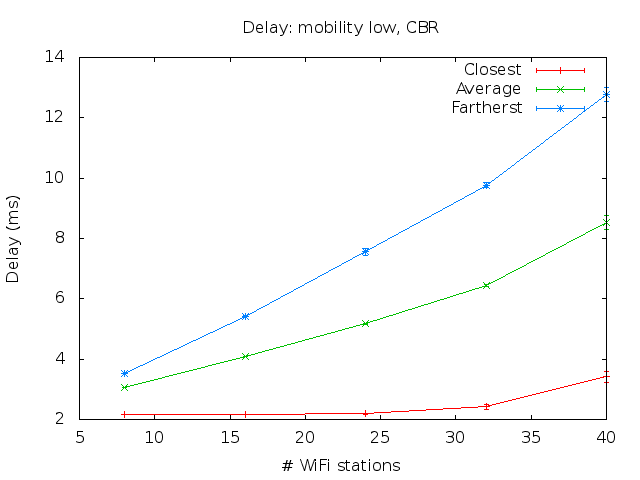
\includegraphics[scale=0.5]{mo818-delay-mob-0-traf-0}
\caption{Gráfico do atraso para mobilidade baixa e CBR}.
\label{fig:atraso-m0-t0}
\end{figure}

\begin{figure}[H]
\centering
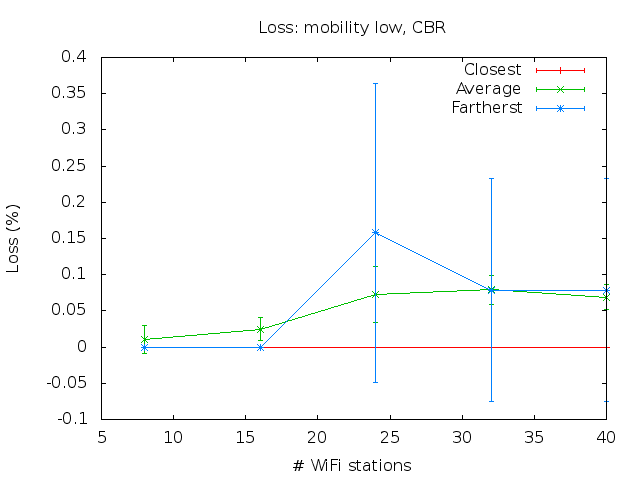
\includegraphics[scale=0.5]{mo818-loss-mob-0-traf-0}
\caption{Gráfico da perda para mobilidade baixa e CBR}.
\label{fig:perda-m0-t0}
\end{figure}

\begin{figure}[H]
\centering
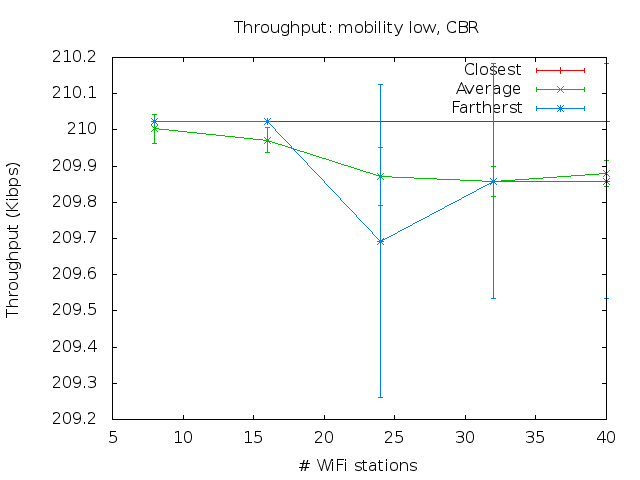
\includegraphics[scale=0.5]{mo818-throughput-mob-0-traf-0}
\caption{Gráfico da vazão para mobilidade baixa e CBR}.
\label{fig:vazao-m0-t0}
\end{figure}

%% Mobilidade Média, CBR
\begin{figure}[H]
\centering
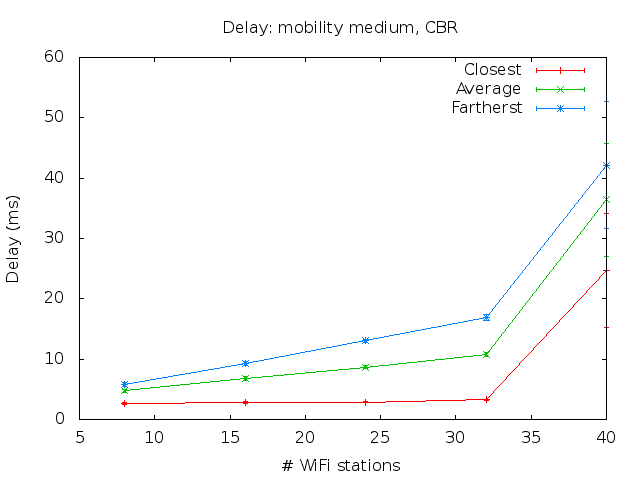
\includegraphics[scale=0.5]{mo818-delay-mob-1-traf-0}
\caption{Gráfico do atraso para mobilidade média e CBR}.
\label{fig:atraso-m1-t0}
\end{figure}

\begin{figure}[H]
\centering
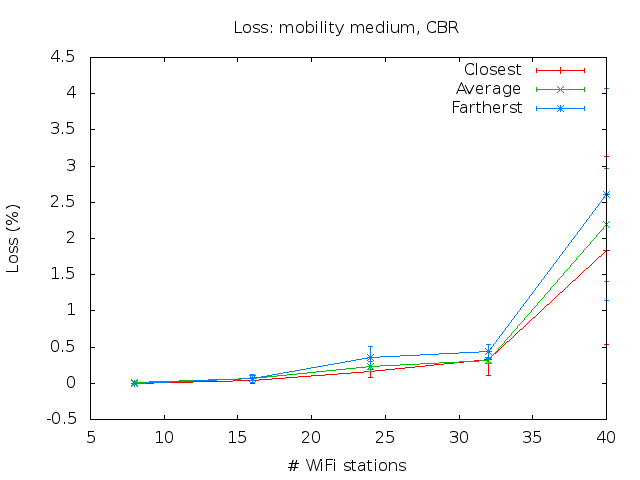
\includegraphics[scale=0.5]{mo818-loss-mob-1-traf-0}
\caption{Gráfico da perda para mobilidade média e CBR}.
\label{fig:perda-m1-t0}
\end{figure}

\begin{figure}[H]
\centering
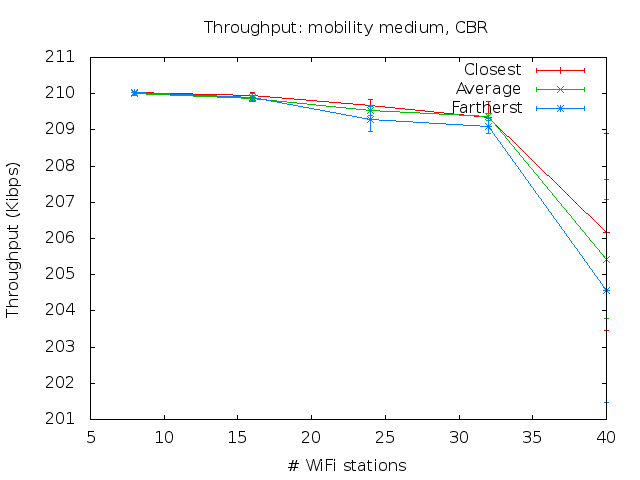
\includegraphics[scale=0.5]{mo818-throughput-mob-1-traf-0}
\caption{Gráfico da vazão para mobilidade média e CBR}.
\label{fig:vazao-m1-t0}
\end{figure}

%% Mobilidade Alta, CBR
\begin{figure}[H]
\centering
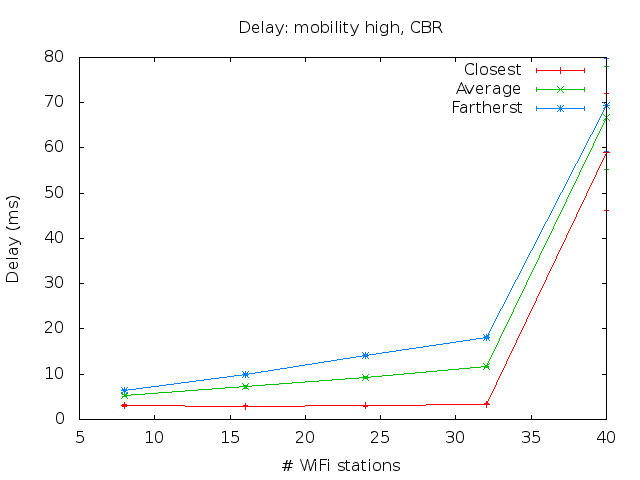
\includegraphics[scale=0.5]{mo818-delay-mob-2-traf-0}
\caption{Gráfico do atraso para mobilidade alta e CBR}.
\label{fig:atraso-m2-t0}
\end{figure}

\begin{figure}[H]
\centering
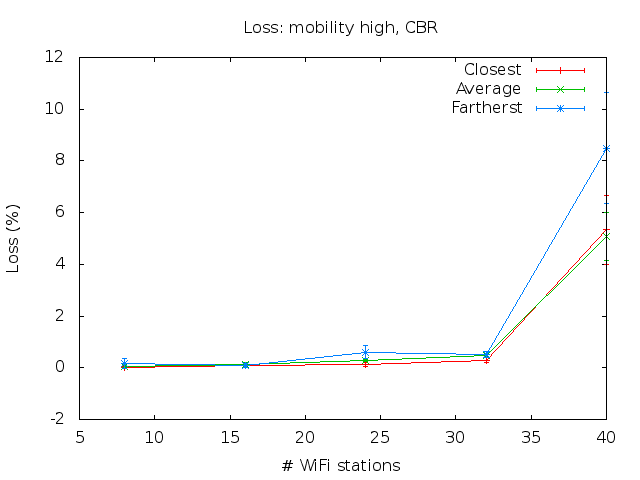
\includegraphics[scale=0.5]{mo818-loss-mob-2-traf-0}
\caption{Gráfico da perda para mobilidade alta e CBR}.
\label{fig:perda-m2-t0}
\end{figure}

\begin{figure}[H]
\centering
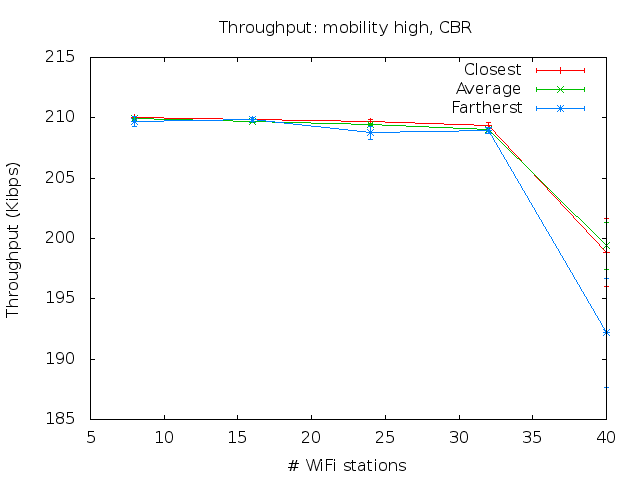
\includegraphics[scale=0.5]{mo818-throughput-mob-2-traf-0}
\caption{Gráfico da vazão para mobilidade alta e CBR}.
\label{fig:vazao-m2-t0}
\end{figure}

%% Mobilidade Baixa, Burst
\begin{figure}[H]
\centering
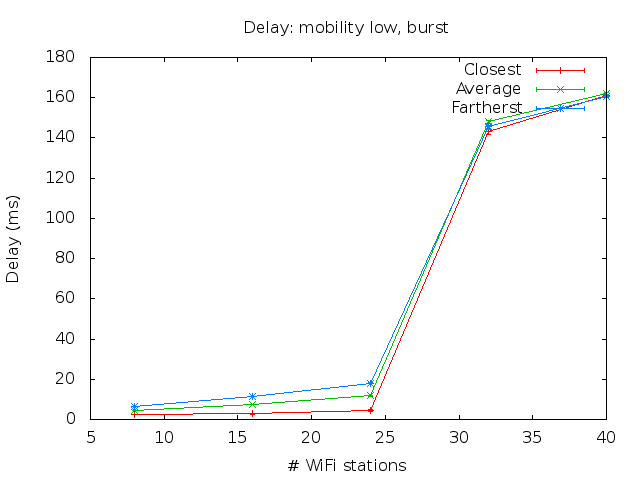
\includegraphics[scale=0.5]{mo818-delay-mob-0-traf-1}
\caption{Gráfico do atraso para mobilidade baixa e rajada}.
\label{fig:atraso-m0-t1}
\end{figure}

\begin{figure}[H]
\centering
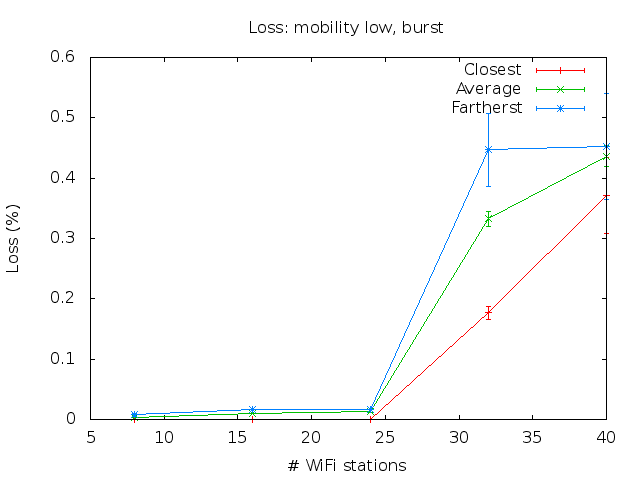
\includegraphics[scale=0.5]{mo818-loss-mob-0-traf-1}
\caption{Gráfico da perda para mobilidade baixa e rajada}.
\label{fig:perda-m0-t1}
\end{figure}

\begin{figure}[H]
\centering
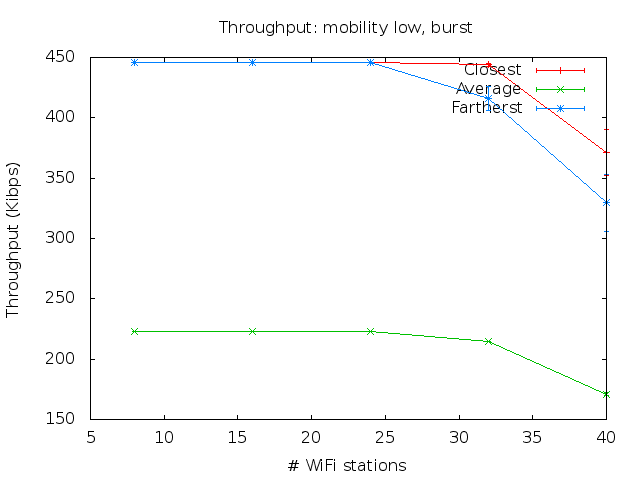
\includegraphics[scale=0.5]{mo818-throughput-mob-0-traf-1}
\caption{Gráfico da vazão para mobilidade baixa e rajada}.
\label{fig:vazao-m0-t1}
\end{figure}

%% Mobilidade Média, Burst
\begin{figure}[H]
\centering
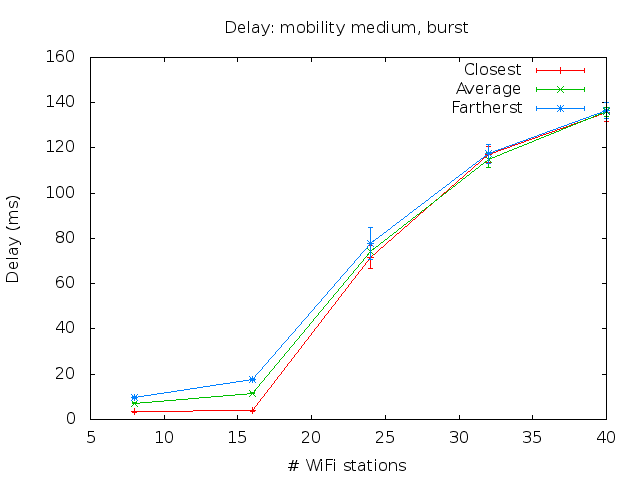
\includegraphics[scale=0.5]{mo818-delay-mob-1-traf-1}
\caption{Gráfico do atraso para mobilidade média e rajada}.
\label{fig:atraso-m1-t1}
\end{figure}

\begin{figure}[H]
\centering
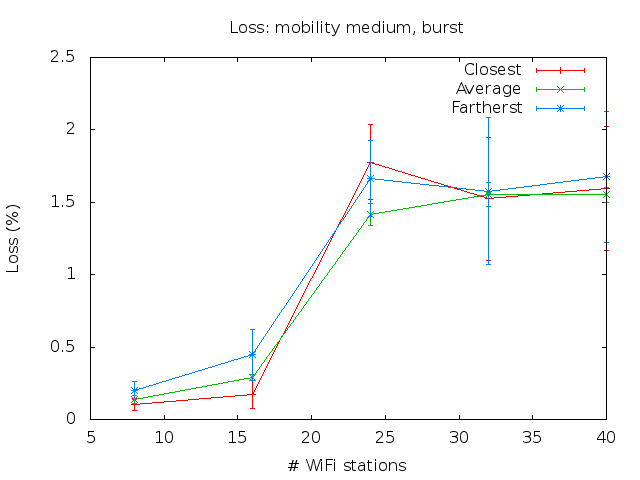
\includegraphics[scale=0.5]{mo818-loss-mob-1-traf-1}
\caption{Gráfico da perda para mobilidade média e rajada}.
\label{fig:perda-m1-t1}
\end{figure}

\begin{figure}[H]
\centering
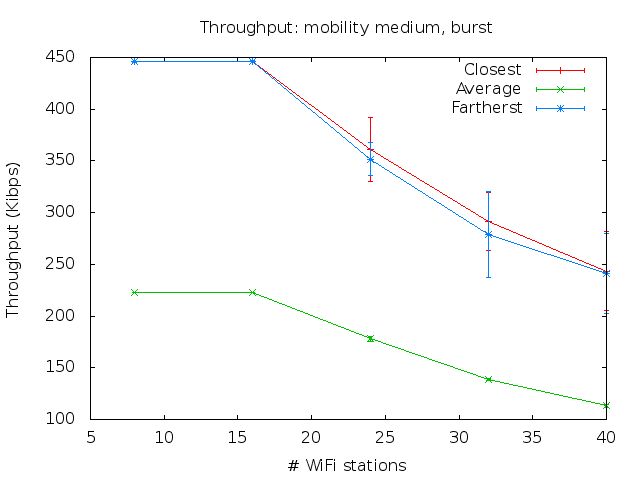
\includegraphics[scale=0.5]{mo818-throughput-mob-1-traf-1}
\caption{Gráfico da vazão para mobilidade média e rajada}.
\label{fig:vazao-m1-t1}
\end{figure}

%% Mobilidade Alta, Burst
\begin{figure}[H]
\centering
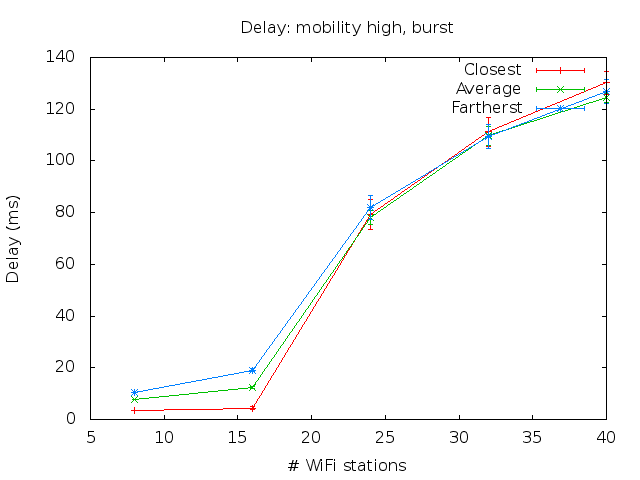
\includegraphics[scale=0.5]{mo818-delay-mob-2-traf-1}
\caption{Gráfico do atraso para mobilidade alta e rajada}.
\label{fig:atraso-m2-t1}
\end{figure}

\begin{figure}[H]
\centering
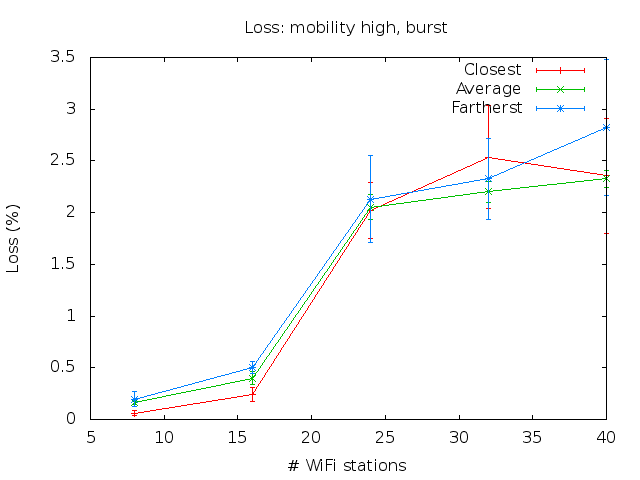
\includegraphics[scale=0.5]{mo818-loss-mob-2-traf-1}
\caption{Gráfico da perda para mobilidade alta e rajada}.
\label{fig:perda-m2-t1}
\end{figure}

\begin{figure}[H]
\centering
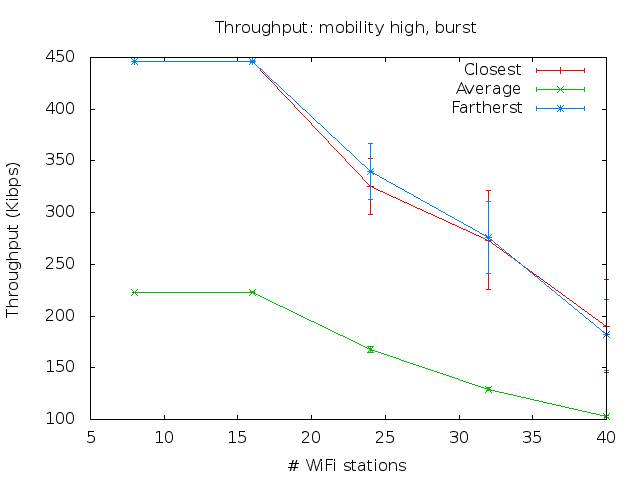
\includegraphics[scale=0.5]{mo818-throughput-mob-2-traf-1}
\caption{Gráfico da vazão para mobilidade alta e rajada}.
\label{fig:vazao-m2-t1}
\end{figure}

\section{Discussão dos Resultados}
\label{sec:02}

\end{document}
